\documentclass[12pt, oneside, titlepage]{article}   	% use "amsart" instead of "article" for AMSLaTeX format

\usepackage{graphicx}
\graphicspath{ {\string} }
\usepackage{subcaption}

%%%%%%%%%%%%%%%%%%%%%%%%%%%%%%%%%%%%%%%%%%%%%%%%%%%%
% set up packages
%%%%%%%%%%%%%%%%%%%%%%%%%%%%%%%%%%%%%%%%%%%%%%%%%%%%
\usepackage{geometry}                
\usepackage{textcomp}                
\usepackage{amsmath}                
\usepackage{graphicx}                
\usepackage{amssymb}                
\usepackage{fancyhdr}                
\usepackage{subcaption}                
\usepackage{bm}                
\usepackage{lineno}
\usepackage{pdfpages}

\usepackage[superscript,noadjust]{cite} % puts dash in citations to abbreviate
\usepackage [autostyle, english = american]{csquotes} % sets US-style quotes

\usepackage{etoolbox} % block quotes

\usepackage{float}
\usepackage{color}

\usepackage{pgf}
\usepackage{tikz}
%\usepackage{eqnarray}

\usepackage{listings} % code blocks
\usepackage{setspace}

\usepackage{lscape}

\usepackage{natbib}
\bibliographystyle{abbrvnat}
\setcitestyle{authoryear,open={(},close={)}}

%%%%%%%%%%%%%%%%%%%%%%%%%%%%%%%%%%%%%%%%%%%%%%%%%%%%
% call packages
%%%%%%%%%%%%%%%%%%%%%%%%%%%%%%%%%%%%%%%%%%%%%%%%%%%%	
\geometry{letterpaper, marginparwidth=60pt} % sets up geometry              		
\linenumbers % adds line numbers 
\MakeOuterQuote{"} % sets quote style
\doublespacing % setspace

%%%%%%%%%%%%%%%%%%%%%%%%%%%%%%%%%%%%%%%%%%%%%%%%%%%%
% patches with etoolbox 
%%%%%%%%%%%%%%%%%%%%%%%%%%%%%%%%%%%%%%%%%%%%%%%%%%%%	
% block quotes
\AtBeginEnvironment{quote}{\small}

% linenumbers
\makeatletter
\patchcmd{\@startsection}{\@ifstar}{\nolinenumbers\@ifstar}{}{}
\patchcmd{\@xsect}{\ignorespaces}{\linenumbers\ignorespaces}{}{}
\makeatother

%%%%%%%%%%%%%%%%%%%%%%%%%%%%%%%%%%%%%%%%%%%%%%%%%%%%
% tikzlibrary modifications
%%%%%%%%%%%%%%%%%%%%%%%%%%%%%%%%%%%%%%%%%%%%%%%%%%%%	
\usetikzlibrary{fit}
\usetikzlibrary{positioning}
\usetikzlibrary{arrows}
\usetikzlibrary{automata}

%%%%%%%%%%%%%%%%%%%%%%%%%%%%%%%%%%%%%%%%%%%%%%%%%%%%
% page formatting; exact 1 in margins
%%%%%%%%%%%%%%%%%%%%%%%%%%%%%%%%%%%%%%%%%%%%%%%%%%%%
\pagestyle{plain}                                                     

\setlength{\textwidth}{6.5in}    
\setlength{\oddsidemargin}{0in}
\setlength{\evensidemargin}{0in}
\setlength{\textheight}{8.5in}
\setlength{\topmargin}{0in}
\setlength{\headheight}{0in}
\setlength{\headsep}{0in}
\setlength{\footskip}{.5in}

%%%%%%%%%%%%%%%%%%%%%%%%%%%%%%%%%%%%%%%%%%%%%%%%%%%%
% defining code blocks using listings package
%%%%%%%%%%%%%%%%%%%%%%%%%%%%%%%%%%%%%%%%%%%%%%%%%%%%

\definecolor{dkgreen}{rgb}{0,0.6,0}
\definecolor{gray}{rgb}{0.5,0.5,0.5}
\definecolor{mauve}{rgb}{0.58,0,0.82}

\lstset{frame=tb,
  language=R,
  aboveskip=3mm,
  belowskip=3mm,
  showstringspaces=false,
  columns=flexible,
  basicstyle={\small\ttfamily},
  numbers=none,
  numberstyle=\tiny\color{gray},
 % keywordstyle=\color{blue},
  commentstyle=\color{dkgreen},
  stringstyle=\color{mauve},
  breaklines=true,
  breakatwhitespace=true,
  tabsize=3,
  otherkeywords={0,1,2,3,4,5,6,7,8,9},
  deletekeywords={data,frame,length,as,character,dunif,ps},
}

%%%%%%%%%%%%%%%%%%%%%%%%%%%%%%%%%%%%%%%%%%%%%%%%%%%%
%%%%%%%%%%%%%%%%%%%%%%%%%%%%%%%%%%%%%%%%%%%%%%%%%%%%
% begin document
%%%%%%%%%%%%%%%%%%%%%%%%%%%%%%%%%%%%%%%%%%%%%%%%%%%%
%%%%%%%%%%%%%%%%%%%%%%%%%%%%%%%%%%%%%%%%%%%%%%%%%%%%

\begin{document}

\bibliographystyle{plainnat} 

\section*{Appendix 1}

% I will use this appendix to compare different models for a success/trial dataset to demonstrate shrinkage due to partial pooling. One of the goals of this appendix is to outline my reasoning for using Bayesian methods to make inferences about vital rates.  

In this appendix, I compare the following models for estimating the probability that seedlings survive to become fruiting plants: (1) maximum likelihood estimates (binomial likelihood), (2) non-hierarchical model with a binomial likelihood with a beta prior, (3) a hierarchical model with a binomial likelihood and year-level parameters on a beta distribution, (4) a hierarchical model with a binomial likelihood and year- and population-level parameters on a beta distribution.

\subsection*{Maximum likelihood estimate}

The following logic underlies how we calculate the maximum likelihood estimate for seedling survival to fruiting. For a single observation, the likelihood that we observe $y$ fruiting plants in a plot if $n$ seedlings were present in the plot can be written as a function of the probability of seedling survival $p$ as $[y|p,n] = \binom{n}{y}p^y(1-p)^{n-y}$. For a set of $N$ observations, each with a number of seedlings $n_i$ and a number of fruiting plants $y_i$ in the $i$th observation, then we can write the likelihood as
%
\begin{align}
  \begin{split}
\mathcal{L} = [\bm{y}|p,\bm{n}]  = \prod_{i=1}^N \binom{n_i}{y_i}p^y_i(1-p)^{n_i-y_i}.
  \end{split}
\end{align}
%
which is often written as
%
\begin{align}
  \begin{split}
\mathcal{L} = [\bm{y}|p,\bm{n}]  = \prod_{i=1}^N \mathrm{binomial}(n_i,p).
  \end{split}
\end{align}
We can use the likelihood to obtain a maximum likelihood estimate (by minimizing the negative log-likelihood). The maximum likelihood estimate $\hat{p}$ is the overall proportion of seedlings that survive to become fruiting plants, summing all the observations. The point is that the proportion calculated in the MATLAB code corresponds to the estimate from a maximum likelihood estimate. Specifically, it calculates a maximum likelihood estimate for each population in each year of the dataset. We thus give each site $j$ and year $k$ its own probability of success $p_{jk}$ and obtain the MLEs $\hat{p}_{jk}$.
%
\begin{align}
  \begin{split}
[\bm{y}|\bm{p},\bm{n}]  = \prod_{j=1}^J\prod_{k=1}^K\prod_{i=1}^N \mathrm{binomial}(n_{ijk},p_{jk}) \label{eq:frequentistMLE}
  \end{split}
\end{align}

\subsection*{Binomial likelihood with a beta prior, complete pooling}

We can turn this into a Bayesian model by adding a prior to our model. Because the beta is a conjugate prior for a binomial distribution, we use use a beta distribution for the prior. In other words, this choice of prior matches the likelihood in a way that the posterior has the same distribution as the prior (cf. Bolker p 177). A beta distribution with shape parameters $\alpha=\beta=1$ corresponds to noninformative prior. For a set of $N$ observations, each with a number of seedlings $n_i$ and a number of fruiting plants $y_i$ in the $i$th observation, we can write the joint posterior as
%
\begin{align}
  \begin{split}
[\bm{y}|p,\bm{n}]  = \prod_{i=1}^N \mathrm{binomial}(n_i,p) \mathrm{beta} (  p | 1 , 1 ).
  \end{split}
\end{align}
%
A single probability $p$ represents the probability of seedling survival to fruiting for the all trials (a model with \textit{complete pooling}). The opposite extreme is a model in which each trial $i$ has its own probability of seedling survival to fruiting $p_i$ (a model with \textit{no pooling}). 
%
\begin{align}
  \begin{split}
[\bm{y}|\bm{p},\bm{n}]  = \prod_{i=1}^N \mathrm{binomial}(n_i,p_i) \mathrm{beta} (  p_i | 1 , 1 ).
  \end{split}
\end{align}
%
To compare our site- and year-specific MLEs to estimates from Bayesian models, we give each site $j$ and year $k$ its own probability of success $p_{jk}$, and place a prior on each $p_{jk}$.
%
\begin{align}
  \begin{split}
[\bm{y}|\bm{p},\bm{n}]  = \prod_{j=1}^J\prod_{k=1}^K\prod_{i=1}^N \mathrm{binomial}(n_{ijk},p_{jk}) \mathrm{beta} (  p_{jk} | 1 , 1 ). \label{eq:bayesianNH}
  \end{split}
\end{align}
%

This is a model in which we are completely pooling observations from each site and year.  Another thing we could say about this model is that it is Bayesian but non-hierarchical. This is extends what happens with the maximum likelihood estimates when we sum across all the plots at a site in a given year and calculate the proportion of seedlings that survive to become fruiting plants. One difference between the two approaches is that with the Bayesian model we account for the number of trials and counts; the data from one plot with a single seedling compromises with the prior to give us posterior probability of success (see \textbf{Comparison}). The Bayesian and frequentist estimates converge as the sample size approaches infinity. 

\subsection*{Binomial model with a beta prior, partial pooling, parameterization via mean: one population, one year}

Next, we'll consider adding pooling to our model. To explain this, we'll focus first on the data from one population in one year. We want a hierarchical model that estimates the probability of survivorship in each plot ($\theta_{i}$) and simultaneously estimates the mean probability of survivorship in the year ($\phi$). The probability of survivorship for each plot $i$ is $\theta_{i}$. We then assume that the probability of survivorship for the $i$ plots is drawn from a distribution of probabilities defined by the mean probability of survivorship in a given year $\phi$ and sample size $\kappa$. This effectively means that the prior on $\theta_{i}$ is itself a parameter; (i.e. we use hyperpriors rather than directly place priors on the probability of survivorship $\theta_{i}$). We reparameterize the beta distribution with its mean $\phi$ and the parameter $\kappa$. The mean of a random variable distributed $\mathrm{beta}(\alpha,\beta)$ is $\phi = \frac{\alpha}{\alpha+\beta}$. With a $\mathrm{beta}(1,1)$ prior, the parameter $\kappa = \alpha + \beta$ is roughly the sample size plus two.
%
\begin{align}
  \begin{split}
[\bm{p},\bm{\theta},\phi,\kappa|\bm{y},\bm{n}]  = & \prod_{i=1}^N \mathrm{binomial}(n_{i},\theta_{i}) 
    \\ & \times \mathrm{beta} (  \theta_{i} | \phi \kappa , (1-\phi) \kappa )
    \\ & \times \mathrm{uniform} ( \phi | 0, 1) \mathrm{Pareto} ( \kappa | 1.5, 1 ). \label{eq:bayesianHyear}
  \end{split}
\end{align}
%
We place a uniform prior on the mean probability of survivorship, $\phi$, because it must lie between 0 and 1. We place a bounded, positive prior on $\kappa$ with the $\mathrm{Pareto}(\alpha,c)$ distribution, which is parameterized by a shape ($\alpha$) and scale ($c$) parameter. 

This parameterization is hierarchical because the estimates for $\phi$ and $\kappa$ contribute to estimates for $\theta_i$. [other effects?]

\subsection*{Binomial model with a beta prior, partial pooling, parameterization via mean: one population, multiple years}

Next, we expand the scope of our analysis to include data from plots ($i$) in multiple years ($j$) of data for a single population $k=1$. Here, we want a hierarchical model that estimates the probability of survivorship in each plot in each year ($\theta_{ij}$). We want to simultaneously estimate the mean probability of survivorship in each year ($\phi_j$) and the mean probability of survivorship in the population. The probability of survivorship for each plot $i$ in a year $j$ is $\theta_{ij}$. We then assume that the probability of survivorship for the $i$ plots in year $j$ is drawn from a distribution of probabilities defined by the mean probability of survivorship in a given year $\phi_j$ and sample size $\kappa_j$. Furthermore, we assume that the mean probability of survivorship in a given year $\phi_j$ is itself drawn from a distribution of probabilities defined by the mean probability of survivorship at the population $\phi_0$ and the parameter $\kappa_0$. 
%
\begin{align}
  \begin{split}
[\bm{p},\bm{\theta},\bm{\phi},\bm{\kappa},\phi_0,\kappa_0|\bm{y},\bm{n}]  = & \prod_{j=1}^J\prod_{i=1}^N \mathrm{binomial}(n_{ij},\theta_{ij}) 
    \\ & \times \mathrm{beta} (  \theta_{ij} | \phi_j \kappa_j , (1-\phi_j) \kappa_j ) 
    \\ & \times \mathrm{beta} (  \phi_{j} | \phi_0 \kappa_0 , (1- \phi_0) \kappa_0 )  \mathrm{Pareto} ( \kappa_j | 1.5, 1 ) 
    \\ & \times \mathrm{uniform} ( \phi_0 | 0 , 1) \mathrm{Pareto} ( \kappa_0 | 1.5, 1 ). \label{eq:bayesianHyearpop} 
      \end{split}
\end{align}
%
This parameterization is hierarchical because the estimates for $\phi_j$ and $\kappa_j$ contribute to estimates for $\theta_{ij}$, and the estimates for $\phi_0$ and $\kappa_0$ contribute to estimates for $\phi_j$. [other effects?]

\subsection*{Binomial model with a beta prior, partial pooling, parameterization via mean: multiple populations, multiple years}

Finally, we expand the scope of our analysis to include data from plots ($i$) in multiple years ($j$) of data for multiple populations $k$. Here, we want a hierarchical model that estimates the probability of survivorship in each plot in each year at each population ($\theta_{ijk}$). We want to simultaneously estimate the mean probability of survivorship in each population $\phi_k$, the mean probability of survivorship in each year ($\phi_jk$). The probability of survivorship for each plot $i$ in a year $j$ at population $k$ is $\theta_{ijk}$. We then assume that the probability of survivorship for the $i$ plots in year $j$ in population $k$ is drawn from a distribution of probabilities defined by the mean probability of survivorship in a given year at a given population $\phi_{jk}$ and paramter $\kappa_{jk}$. Furthermore, we assume that the mean probability of survivorship in a given year in a given population $\phi_{jk}$ is itself drawn from a distribution of probabilities defined by the mean probability of survivorship for the population $\phi_{0,k}$ and the parameter $\kappa_{0,k}$. The model is similar to the one for one population except the indexing has changed so that we estimate a mean probability of survivorship for each population.
%
\begin{align}
  \begin{split}
[\bm{p},\bm{\theta},\bm{\phi},\bm{\kappa},\phi_0,\kappa_0|\bm{y},\bm{n}]  = & \prod_{k=1}^K\prod_{j=1}^J\prod_{i=1}^N \mathrm{binomial}(n_{ijk},\theta_{ijk}) 
    \\ & \times \mathrm{beta} (  \theta_{ijk} | \phi_{jk} \kappa_{jk} , (1-\phi_{jk}) \kappa_{jk} ) 
    \\ & \times \mathrm{beta} (  \phi_{jk} | \phi_{0,k} \kappa_{0,k} , (1- \phi_{0,k}) \kappa_{0,k} )  \mathrm{Pareto} ( \kappa_j | 1.5, 1 ) 
    \\ & \times \mathrm{uniform} ( \phi_{0,k} | 0 , 1) \mathrm{Pareto} ( \kappa_{0,k} | 1.5, 1 ). 
  \end{split}
\end{align}
%
This parameterization is hierarchical because the estimates for $\phi_{jk}$ and $\kappa_{jk}$ contribute to estimates for $\theta_{ijk}$, and the estimates for $\phi_{0,k} $ and $\kappa_{0,k} $ contribute to estimates for $\phi_{jk}$. [other effects?]

\iffalse
\subsection*{Binomial model with a beta prior, partial pooling}

Next, we'll consider adding pooling to our model. We do this by putting hyperpriors on the parameters for the beta distribution. Focusing first on one population, we give the population a per-year probability of success $p_k$. We place a prior on each $p_{k}$ but rather than directly parameterize the probability of success we use hyperpriors. We'll use the parameterization in Kruschke:
%
\begin{align}
  \begin{split}
[\bm{p},\omega,\kappa|\bm{y},\bm{n}]  = & \prod_{k=1}^K\prod_{i=1}^N \mathrm{binomial}(n_{ik},p_{k}) 
    \\ & \times \mathrm{beta} (  p_{k} | \omega(\kappa-2) +1 , (1-\omega) (\kappa -2) + 1) 
    \\ & \times \mathrm{beta} ( \omega | 1, 1) \mathrm{gamma} ( \kappa | 0.01, 0.01)  .
  \end{split}
\end{align}
%
This parameterization is hierarchical and we can use it to illustrate one of the effects of using this structure in our models. Let's pick a population with years in which there were few data points. For the purposes of illustration, we choose to work with the Lucas Creek East (LCE) population here. We fit the model above to the data from LCE and plot the posteriors for the parameter $\omega$ in Figure~\ref{fig:hierarchical-1}, which corresponds to the mode of the beta distribution. The figure illustrates the concept of \textit{shrinkage}; the posterior distributions of year-level $\theta_k$ are pulled towards the population-level mode $\omega$. This effect is particularly evident in years in which there are few data points (number of samples in each year, from 2006-2015: 20, 7, 17, 14, 19, 1, 1, 3, 1, 8). In Figure~\ref{fig:hierarchical-1}, this is shown by the overlap between the posterior distribution for $\omega$ and $\theta_k$ for years $k$ in which there are few data points. This is particularly true in 2011--2014. One important effect of this is that the [variance between estimated values $\theta_k$ is less than the variance between the individual proportions correct] (paraphrasing Kruschke)

 \begin{figure}[h]
   \centering
  %#\begin{tabular}{@{}c@{\hspace{.5cm}}c@{}}
       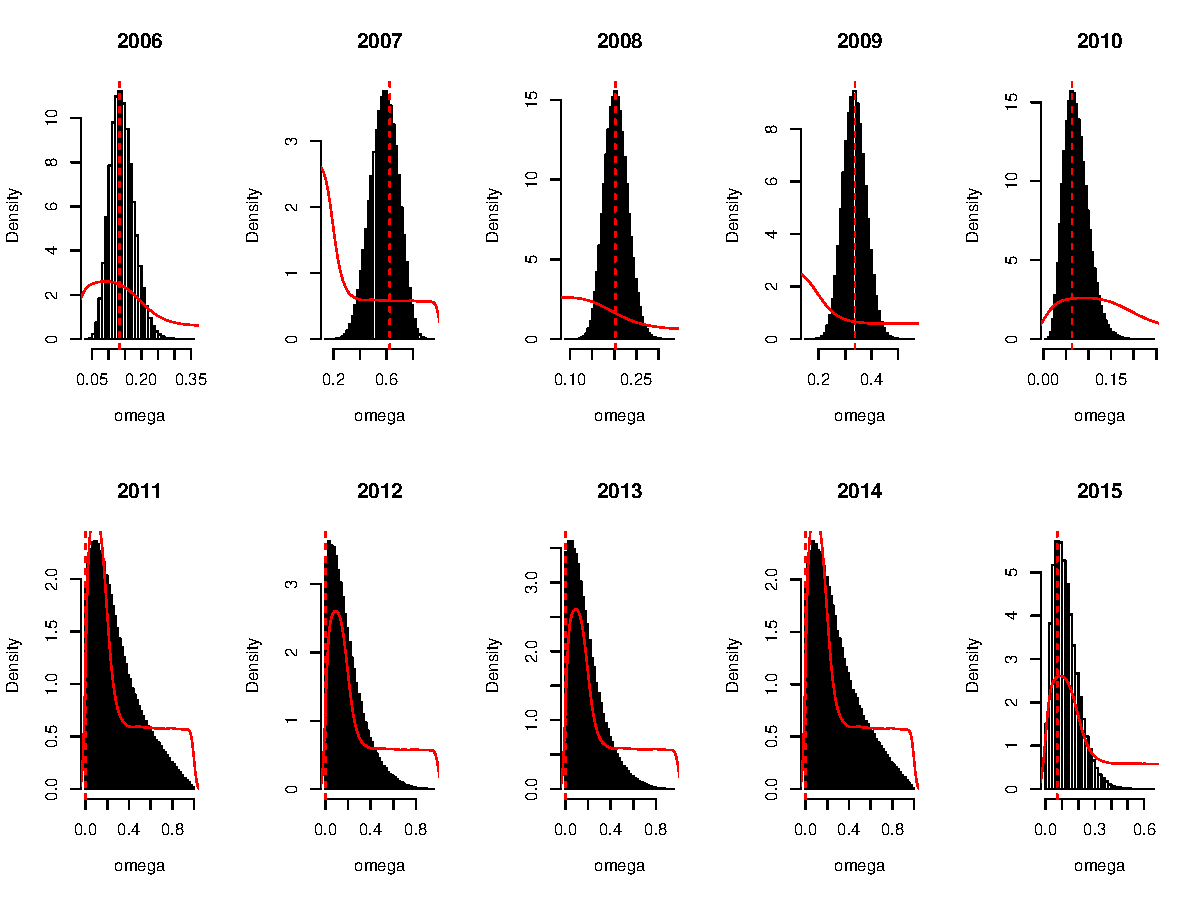
\includegraphics[page=1,width=.9\textwidth]{../figures/appendix-x-hierarchical}  
    \caption{ The posterior distribution for $\theta_k$ for a model fitted to data from Lucas Creek East. The histogram represents draws from the posterior distribution. The vertical, dotted red line indicates the total proportion of successes (fruiting plants/seedlings) in each year. The solid red line is the density of draws from the posterior of $\omega$. }
 \label{fig:hierarchical-1}
\end{figure}

For comparison, we also fit the same model to data from the Black Gulch (BG) population. For BG, most years have a higher number of data points (number of samples in each year, from 2006-2015: 18, 20, 21, 26, 23, 26, 20, 23, 3, 26). Here, it's clear that most posterior distributions for year-level $\theta_k$ are not greatly influenced by the population-level mode $\omega$. 

 \begin{figure}[h]
   \centering
  %#\begin{tabular}{@{}c@{\hspace{.5cm}}c@{}}
       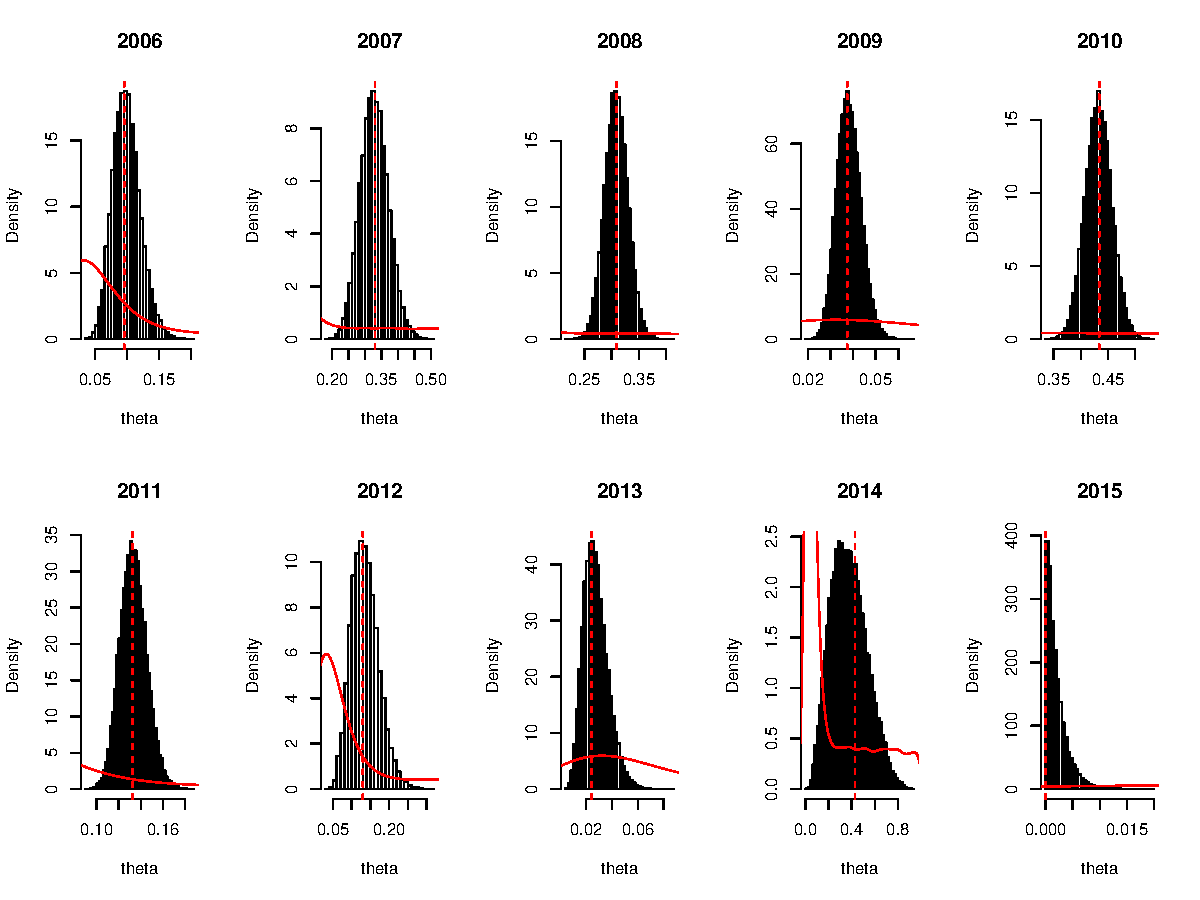
\includegraphics[page=1,width=.9\textwidth]{../figures/appendix-x-hierarchicalBG}  
    \caption{ The posterior distribution for $\theta_k$ for a model fitted to data from Black Gulch. The histogram represents draws from the posterior distribution. The vertical, dotted red line indicates the total proportion of successes (fruiting plants/seedlings) in each year. The solid red line is the density of draws from the posterior of $\omega$. }
 \label{fig:hierarchical-2}
\end{figure}

To compare our population- and year-specific estimates, we give each population $j$ and year $k$ its own probability of success $p_{jk}$, place priors $\omega_j$ and $\kappa_j$ on each $p_{jk}$, and give each prior a set of hyperpriors.
%
\begin{align}
  \begin{split}
[\bm{p},\omega,\kappa|\bm{y},\bm{n}]  = & \prod_{k=1}^K\prod_{i=1}^N \mathrm{binomial}(n_{ik},p_{jk}) 
    \\ & \times \mathrm{beta} (  p_{jk} | \omega_j(\kappa_j-2) +1 , (1-\omega_j) (\kappa_j -2) + 1) 
    \\ & \times \mathrm{beta} ( \omega_j | 1, 1) \mathrm{gamma} ( \kappa_j | 0.01, 0.01)  .
  \end{split}
\end{align}
%
Effectively, this is a model in which we are partially pooling observations from each population. The posterior estimates for $p_jk$ from this model are similar to one in which observations from each population are completely pooled. When there are few data points, the population-level paramater $\omega_j$ has an effect on the population- and year-level $\theta_jk$ (see \textbf{Comparison}).

\subsection*{Multi-level binomial model with partial pooling and a beta prior}

Next, we could consider pooling across all sites and years in our dataset. We would this by putting hyperpriors on the parameters for the beta distribution. This means that we estimate parameters for all populations and years simultaneously. There is a parameter $\omega_j$ that determines the mode of each population, $\omega$ that determines the mode across all populations, $\kappa_j$ that determines the concentration of the data between years, and $\kappa$ that determines the concentration of data at each population. We are interested in the mean at each site. We'll use the parameterization in Kruschke:
%
\begin{align}
  \begin{split}
[\bm{p},\omega,\kappa|\bm{y},\bm{n}]  = & \prod_{j=1}^J \prod_{k=1}^K \prod_{i=1}^N \mathrm{binomial}(n_{ijk},p_{jk}) 
    \\ & \times \mathrm{beta} (  p_{jk} | \omega_j(\kappa_j-2) +1 , (1-\omega_j) (\kappa_j -2) + 1) 
    \\ & \times \mathrm{beta} ( \omega_j |  \omega(\kappa-2) +1 , (1-\omega) (\kappa -2) + 1) \mathrm{gamma} ( \kappa_j | .01, .01) 
    \\ & \times \mathrm{beta} ( \omega | 1 , 1 )  \mathrm{gamma} ( \kappa | .01, .01)  .
  \end{split}
\end{align}

I'm going to leave this out for the time being. This would 100\% be a future direction!
\fi

\subsection*{Hierarchical model parameterization}

I considered four parameterizations for the structure of the hierarchical model. The first is a parameterization of the mean probability of success and the sample size. The second is a parameterization in which I moment match the parameters of the beta distribution. The third is a parameterization in which I use a logit-link function and a centered parameterization. The fourth is a parameterization in which I use a logit-link function and a non-centered parameterization. 

\subsubsection*{Hierarchical model with parameterization for beta distribution by mean probability of success, $\phi$ and sample size, $\kappa$.}
\begin{align}
  \begin{split}
[\bm{\theta},\mu,\nu|\bm{y},\bm{n}]  = & \prod_{i=1}^N \mathrm{binomial}(y_{i}|n_{i},\theta_{i}) 
    \\ & \times \mathrm{beta} (  \theta_{i} | \phi \kappa , (1-\phi) \kappa )
    \\ & \times \mathrm{uniform} ( \phi | 0, 1) \mathrm{Pareto} ( \kappa | 1.5, 1 )
  \end{split}
\end{align}
%
\subsubsection*{Hierarchical model with parameterization of beta distribution by moment matching mean and variance.}
\begin{align}
  \begin{split}
[\bm{\theta},\mu,\sigma|\bm{y},\bm{n}]  = & \prod_{i=1}^N \mathrm{binomial}(y_{i}|n_{i},\theta_{i}) 
    \\ & \times \mathrm{beta} (  \theta_{i} | \frac{\mu^2 - \mu^3 - \mu \times \sigma^2}{\sigma^2} , \frac{\mu - 2 \times \mu^2 + \mu^3 - \sigma^2 + \mu \times \sigma^2}{\sigma^2} )
    \\ & \times \mathrm{normal} ( \mu | 0, 1) \mathrm{Half-Cauchy} ( \sigma | 0, 1 )
   \end{split}
\end{align}
%
\subsubsection*{Hierarchical model with parameterization via log-odds probability of success, centered.}
\begin{align}
  \begin{split}
[\bm{\theta},\bm{\alpha},\mu,\sigma|\bm{y},\bm{n}]  = & \prod_{i=1}^N \mathrm{binomial}(y_{i}|n_{i},\mathrm{logit}^-1(\alpha_i)) 
    \\ & \times \mathrm{normal} (  \alpha_{i} | \mu, \sigma )
    \\ & \times \mathrm{normal} ( \mu | 0, 1) \mathrm{Half-Cauchy} ( \sigma | 0, 1 )
   \end{split}
\end{align}
where
\begin{align}
  \begin{split}
\theta_i = \mathrm{logit}^-1(\alpha_i)
   \end{split}
\end{align}
%
\subsubsection*{Hierarchical model with parameterization via log-odds probability of success, non-centered.}
\begin{align}
  \begin{split}
[\bm{\theta},\bm{\alpha},\mu,\sigma|\bm{y},\bm{n}]  = & \prod_{i=1}^N \mathrm{binomial}(y_{i}|n_{i},\mathrm{logit}^-1(\alpha_i)) 
    \\ & \times \mathrm{normal} (  \alpha^{std}_i | 0 , 1 )
    \\ & \times \mathrm{normal} ( \mu | 0, 1) \mathrm{Half-Cauchy} ( \sigma | 0, 1 ) 
   \end{split}
\end{align}
where
\begin{align}
  \begin{split}
\theta_i = \mathrm{logit}^-1(\alpha_i) \\
\alpha_i = \mu + \alpha^{std}_{i} \times \sigma
   \end{split}
\end{align}

\subsection*{Comparison}

First, we want to explore estimates from a Bayesian model compare to the maximum likelihood estimates. Second, we want to explore the effect of adding hierarchical structure to the parameter estimates in our models. Finally, we want to explore the effect of adding hierarchical structure on how appropriate our models are (compare posterior predictive checks).

\subsubsection*{Estimates from maximum likelihood versus Bayesian models} 

First, we want to explore estimates from a Bayesian model compare to the maximum likelihood estimates. The comparison I am interested in is the effect of adding a prior, rather than the effect of adding hierarchy to the model. I will compare the maximum likelihood estimates (equation~\eqref{eq:frequentistMLE}) and the non-hierarchical Bayeisan model (equation~\eqref{eq:bayesianNH}). The first panel in Figure~\ref{fig:mle_bayes} shows that the maximum likelihood estimates are pretty similar to those from the Bayesian model with complete pooling per population and a beta-binomial parameterization. The major differences are where the maximum likelihood estimates approach 0 or 1. The second panel in Figure~\ref{fig:mle_bayes} shows that this is because those estimates come from year-population combinations with a small sample size. For example, the MLE for a year-population combination with one plot and 1 seedling that dies before fruiting would be 0. In the Bayesian model, the prior has a comparatively larger influence on the posterior in situations where there is little data. In this case, the posterior would be a compromise between our one data point and our prior. The estimates converge once we have ~5 data points.

\subsubsection*{Hierarchical structure}

Second, we want to explore the effect of adding hierarchical structure to the parameter estimates in our models. These comparisons will all be among models fit to data for one population ($k=1$). I am interested in comparing a non-hierarchical model (equation~\eqref{eq:bayesianNH}), a hierarchical model with year-level parameters (equation~\eqref{eq:bayesianHyear}), and a hierarchical model with year-level and population-level parameters (equation~\eqref{eq:bayesianHyearpop}). All these comparisons are made at a randomly selected site. 

The first panel in figure~\ref{fig:hierarchical_shrinking1} shows that the complete pooling model produces estimates for each plot that are identical; there is one estimate per year. The second and third panels show taht the posterior medians for $\theta_i$ and $\theta_{ij}$ from the hierarchical models are 'shrunk' from the point estimates $y_{ij}/n_{ij}$ towards the year-level mean (dotted line). Figure~\ref{fig:hierarchical_shrinking2} that the models shrink $\theta_i$ and $\theta_{ij}$ towards the year-level estimate, and that this effect varies across years. 

In the non-hierarchical model, the posterior distribution for the probability of survivorship in each year is $p_{jk}$ (where $k$=1) in equation~\eqref{eq:bayesianNH}). In the hierarchical model with year-level parameters, the posterior distribution for the mean probability of survivorship in each year is $\phi$ in equation~\eqref{eq:bayesianHyear}. In the hierarchical model with year- and population-level parameters, the posterior distribution for the mean probability of survivorship in each year is $\phi_j$, and the posterior distribution for the mean probability of survivorship in the population is $\phi_0$ in equation~\eqref{eq:bayesianHyearpop}. Figures~\ref{fig:hierarchyPosteriors_nh_hyear}) and~\ref{fig:hierarchyPosteriors_nh_hyearpop}) both show that the posterior distribution for the mean-probability of survivorship from the hierarchical models (red lines) is broader than for the probability of survivorship from the non-hierarchical model (blue lines). Figure~\ref{fig:hierarchyPosteriors_nh_hyearpop}) also shows the posterior for the population-level probability of survivorship (black line).

Figure~\ref{fig:hierarchyPosteriorsSummary}) summarizes the posterior distributions for the year-level probability of survivorship by their median and 95\% credible intervals. The hierarchical structure has the effect of broadening the credible intervals associated with the estimated mean probability of survivorship in each year. 
 
\subsubsection*{Model parameterization}
I compare a few key properties of these fits to provide a sense of which parameterization is most efficient here. First, look at the relationship of hyperparameters. Second, look at the number of effective samples. Third, look at the amount of shrinkage from each model fit. Fourth, compare the population-level estimates from each of the models. 

Figure X shows how these different parameterizations sample hyperparameter space, and correlations between hyperparameters and probability of success. Uncorrelated sampling suggests the parameterization is exploring parameter space. 'Funnels' in correlations between probability of sucess and hyperparameters indicate that particular parameter combinations are undersampled. Figure X shows that the parameterizations can vary in how efficiently they sample. Each model was run for an identical number of iterations; in this figure, I compare the number of effective samples obtained for each $\theta_i$. Figure X illustrates an important general feature of hierarchical models; pooling is greater when there are fewer trials. The right panel in the figure also demonstrates that the amount of shrinkage varies between parameterizations. The next figure shows the same points; the mean and sample size parameterization is the least shrunk towards the population mean (denoted by the dashed line). Finally, Figure X shows that the median population-level estimates for the different parameterizations are similar but that they differ in how broad the credible intervals are. The log-odds parameterization imposes greater shrinkage around the population mean, leading to narrower credible intervals over the mean and sample size parameterization.  
 
\subsubsection*{Posterior predictive checks}
 
Finally, we want to explore the effect of adding hierarchical structure on how appropriate our models are (compare posterior predictive checks). The figures appended to this PDF (still need to figure out how to best integrate them) show graphical posterior predictive checks (cf. Gabry et al. 2019) for the non-hierarchical (blue), the hierarchical with year-level parameters (purple), and the hierarchical with year- and population-level parameters (gray). Gabry et al. (2019) describe how to perform PPCs: the posterior distribution is used to  simulate data, and this data is summarized and compared to observed test statistics. For all three models, the mean of simulations from the posterior does a good job matching the observed mean from the data. This is perhaps not surprising because the models are parameterized via the mean probability of success. Posterior predictive checks for the variance may be more informative (variance is not a parameter in our models). The variance of simulations from the posterior of the non-hierarchical model under- or over-estimates the variance. The variance of simulations from both the hierarchical models do a reasonable job at matching the observed variance. 


% Figure~\ref{fig:complete_vs_partial} shows that, when the data are fit at the population-level only, a model with complete and partial pooling give fairly similar estimates. The difference between the posterior for a model with complete versus partial pooling has a greater range for smaller sample sizes (CIs are larger for smaller sample sizes) and a model with complete pooling returns slightly higher estimates. Figures~\ref{fig:match} and~\ref{fig:mismatch} compare the posterior distribution for population- and year-combinations with many data points (30 data points in Figure~\ref{fig:match}) and few data points (1 data point in Figure~\ref{fig:mismatch}). When there are few data points, the posterior for $p_{jk}$ in the partial pooling model is influenced by the population-level parameter $\omega$ (Figure~\ref{fig:mismatch}).


%Goal is to compare the output from each of these models. They should be pretty similar for most of the data because it's well-replicated and the sample sizes are reasonable. The differences that I am interested in pointing out are

%- what happens when there are few observations (the prior has influence)
%- how well can we estimate the site mean or the year mean from each dataset?
%- prediction: which of our datasets does a better job at predicting?

\clearpage

 \begin{figure}[h]
   \centering
  %#\begin{tabular}{@{}c@{\hspace{.5cm}}c@{}}
       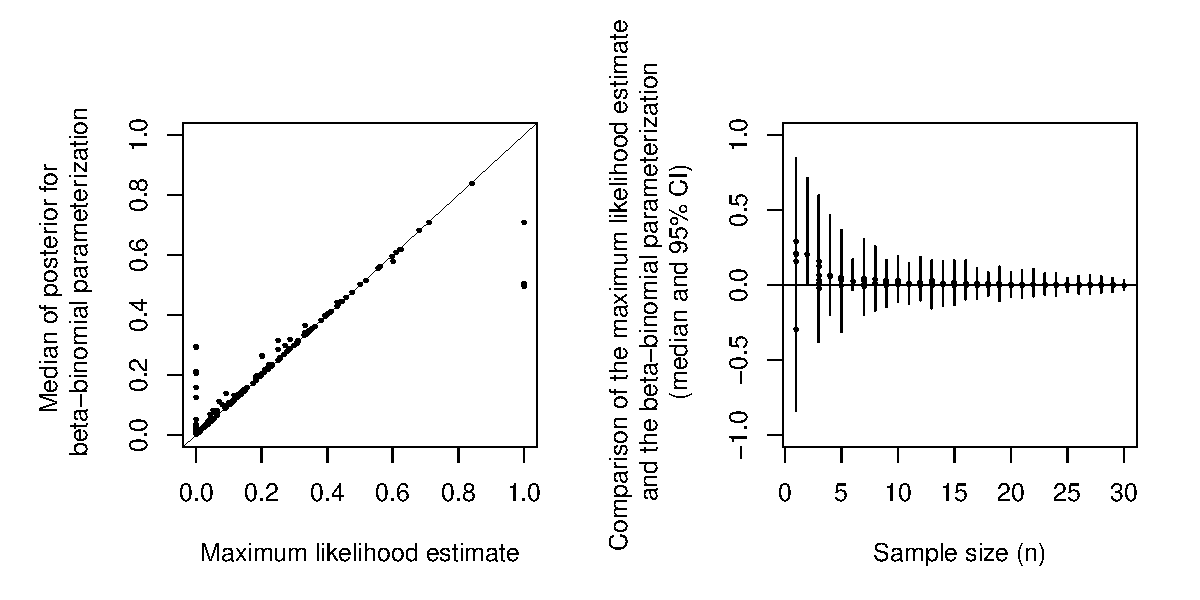
\includegraphics[page=1,width=.9\textwidth]{../figures/appendix-x-mle_bayes}  
    \caption{ (A) This panel plots the median of the posterior from the beta-binomial with complete pooling per population against the maximum likelihood estimate. (B) This panel compares the full posterior distribution from the beta-binomial parameterization with the maximum likelihood estimate. The plot shows the median of the difference (with 95\% CIs) against the sample size in the year-population combination for that estimate.  }
 \label{fig:mle_bayes}
\end{figure}

\begin{figure}[h]
   \centering
  %#\begin{tabular}{@{}c@{\hspace{.5cm}}c@{}}
       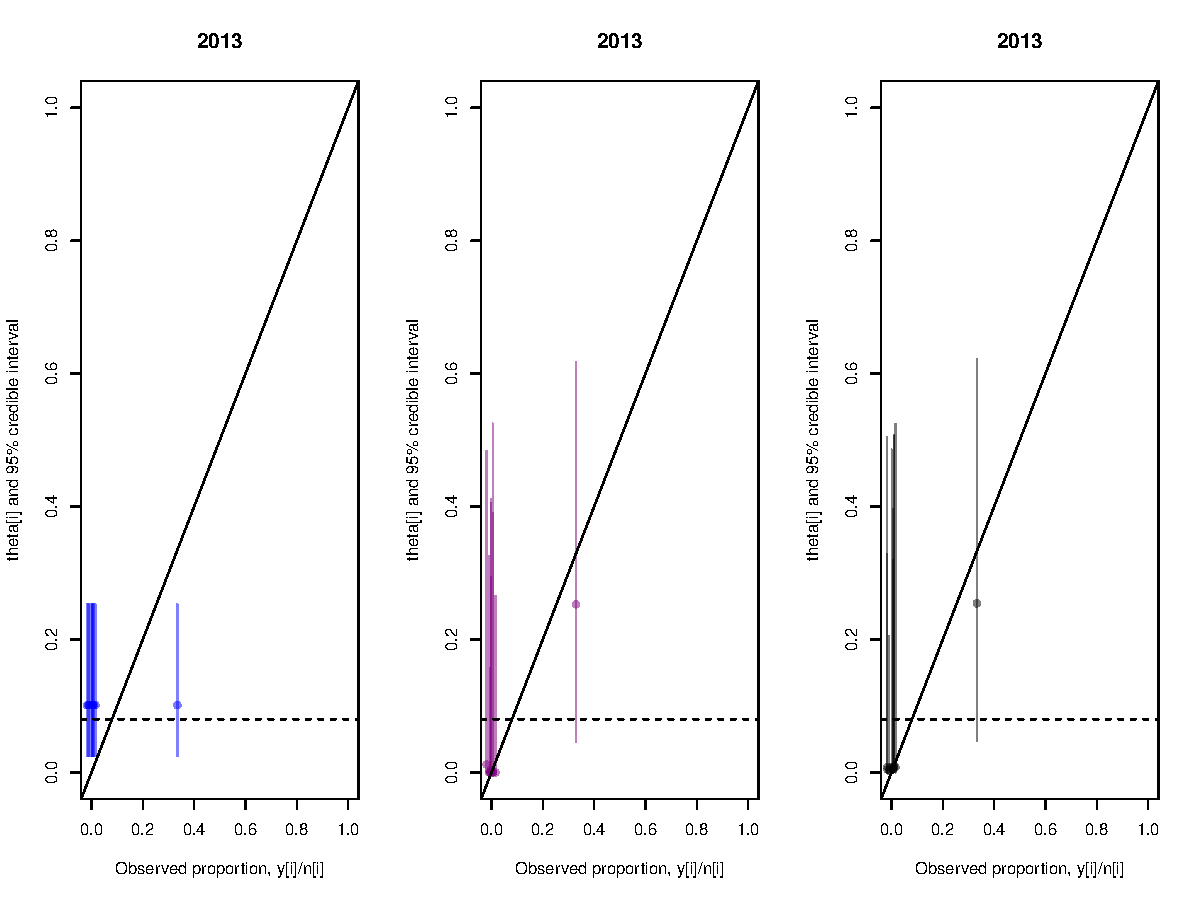
\includegraphics[page=1,width=.9\textwidth]{../figures/appendix-x-figure54-2}  
    \caption{ Posterior median and 95\% credible intervals for a randomly selected year, based on simulations from the joint posterior distribution plotted against the unpooled estimates. The 1:1 line corresponds to unpooled estimates $\theta_i = y_i/n_i$. The horizontal, dashed line corresponds to the year-level maximum likelihood estimate. (A) Estimates from the complete pooling model. (B) Estimates from the hierarchical model with year-level parameters. (C) Estimates from the hierarchical model with year- and population-level parameters. } 
 \label{fig:hierarchical_shrinking1}
\end{figure}

\begin{figure}[h]
   \centering
  %#\begin{tabular}{@{}c@{\hspace{.5cm}}c@{}}
       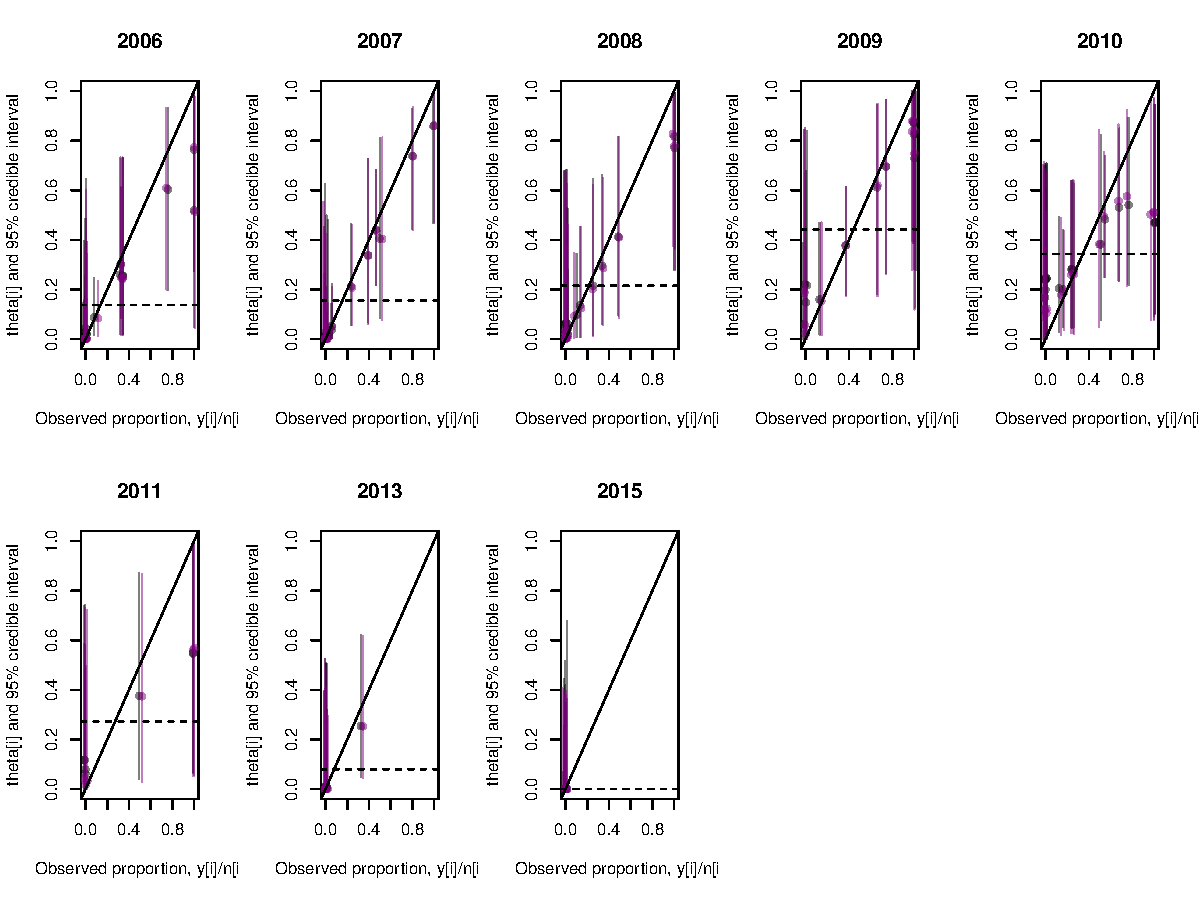
\includegraphics[page=1,width=.9\textwidth]{../figures/appendix-x-figure54}  
    \caption{ (A) Posterior median and 95\% credible intervals for a randomly selected year, based on simulations from the joint posterior distribution plotted against the unpooled estimates. The 1:1 line corresponds to unpooled estimates $\theta_i = y_i/n_i$. The horizontal, dashed lines corresponds to the year-level maximum likelihood estimates. } 
 \label{fig:hierarchical_shrinking2}
\end{figure}


 \begin{figure}[h]
   \centering
  %#\begin{tabular}{@{}c@{\hspace{.5cm}}c@{}}
       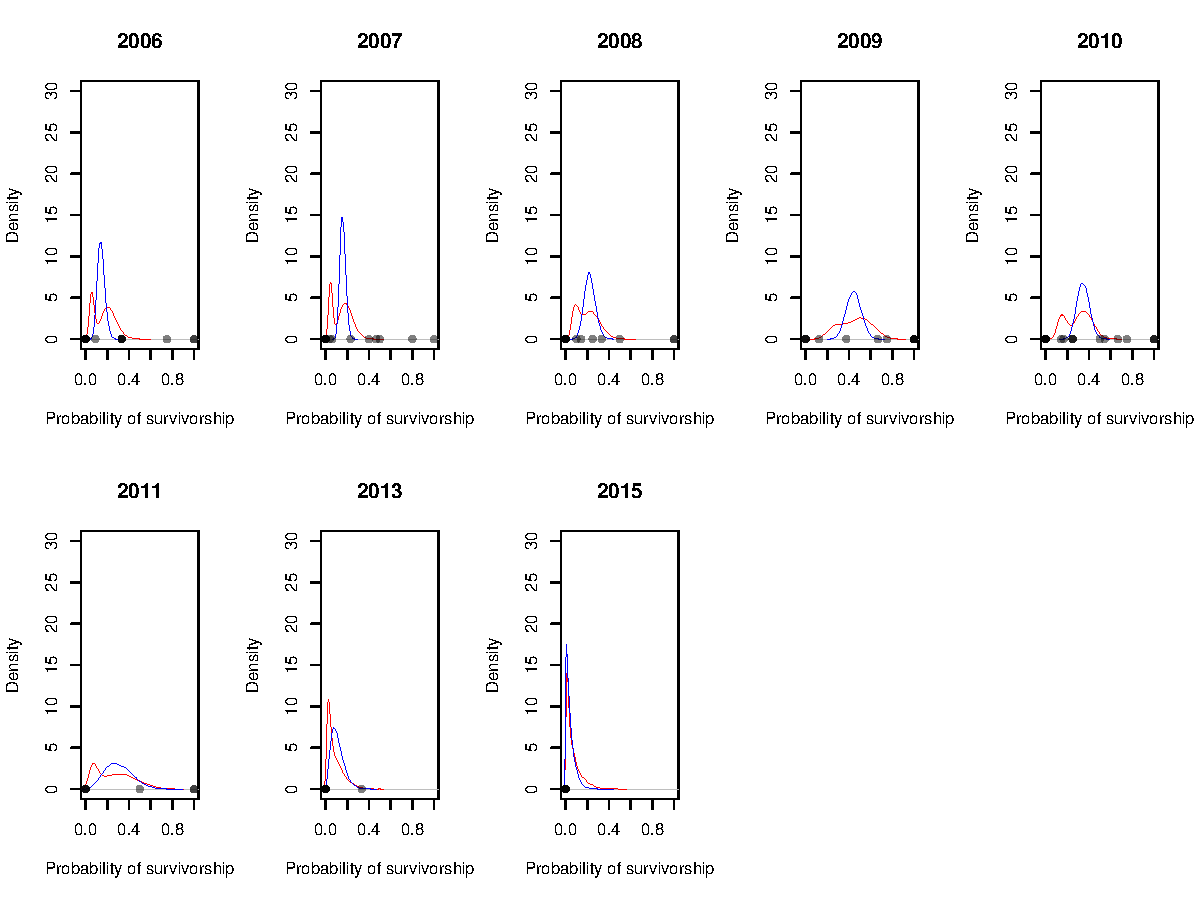
\includegraphics[page=1,width=.9\textwidth]{../figures/appendix-x-hierarchyPosteriors_nh_hyear}  
    \caption{ (A) Comparison of and nonhierarchical (blue) and year-level parameter hierarchical (red) model. The curves are posterior density distributions for the probability of survivorship $p_{jk}$ (blue) and $\phi$ (red). } 
 \label{fig:hierarchyPosteriors_nh_hyear}
\end{figure}

\begin{figure}[h]
   \centering
  %#\begin{tabular}{@{}c@{\hspace{.5cm}}c@{}}
       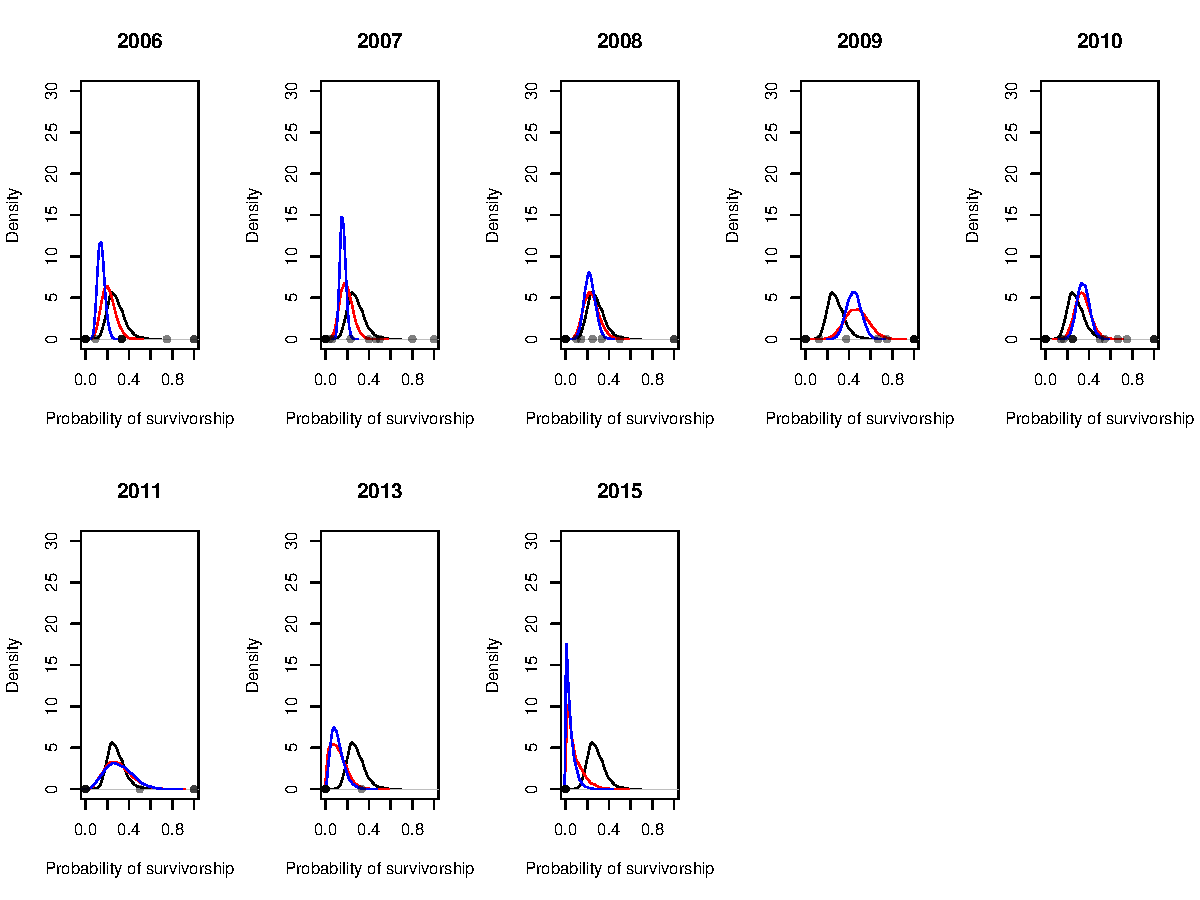
\includegraphics[page=1,width=.9\textwidth]{../figures/appendix-x-hierarchyPosteriors_nh_hyearpop}  
    \caption{ (A) Comparison of and nonhierarchical and year- and population-level parameter hierarchical model.  The curves are posterior density distributions for the probability of survivorship $p_{jk}$ (blue), $\phi_j$ (red), and $\phi_0$ (black).  }
 \label{fig:hierarchyPosteriors_nh_hyearpop}
\end{figure}


 \begin{figure}[h]
   \centering
  %#\begin{tabular}{@{}c@{\hspace{.5cm}}c@{}}
       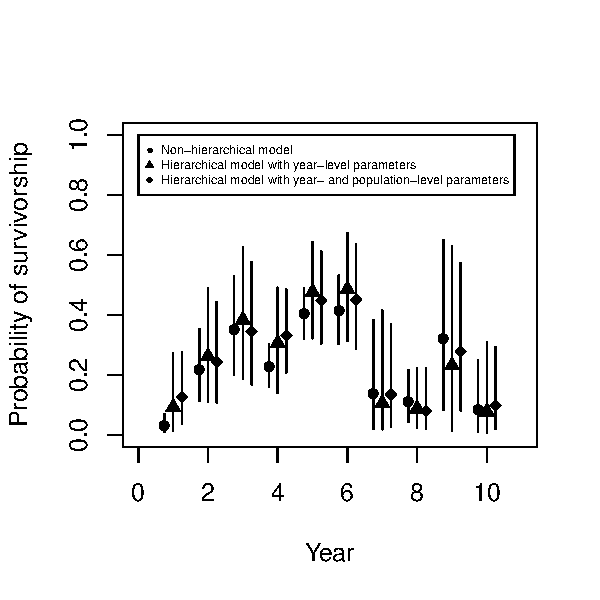
\includegraphics[page=1,width=.9\textwidth]{../figures/appendix-x-hierarchyPosteriorsSummary}  
    \caption{ (A) Comparison of median and 95\% confidence intervals for models with three levels of structure, fit to the same dataset.   }
 \label{fig:hierarchyPosteriorsSummary}
\end{figure}

\clearpage


\includepdf[pages={2,3,4},fitpaper=true]{../figures/appendix-x-ppc.pdf}

\includepdf[pages={5,6,7},fitpaper=true]{../figures/appendix-x-ppc.pdf}



\iffalse
 \begin{figure}[h]
   \centering
  %#\begin{tabular}{@{}c@{\hspace{.5cm}}c@{}}
       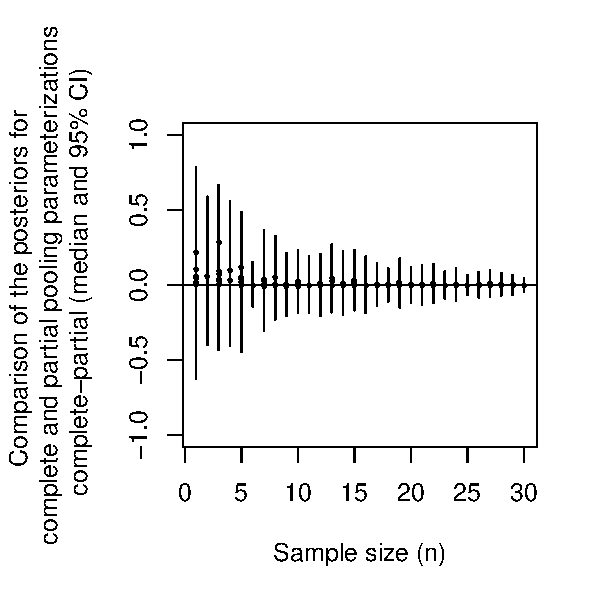
\includegraphics[page=1,width=.9\textwidth]{../figures/appendix-x-bayescomp_bayeshier}  
    \caption{ (A) This plot compares the full posterior distribution of the beta-binomial parameterization with complete pooling against the beta-binomial parameterization with partial pooling. The plot shows the median of the difference (with 95\% CIs) against the sample size in the year-population combination for that estimate.  }
 \label{fig:complete_vs_partial}
\end{figure}


 \begin{figure}[h]
   \centering
  %#\begin{tabular}{@{}c@{\hspace{.5cm}}c@{}}
       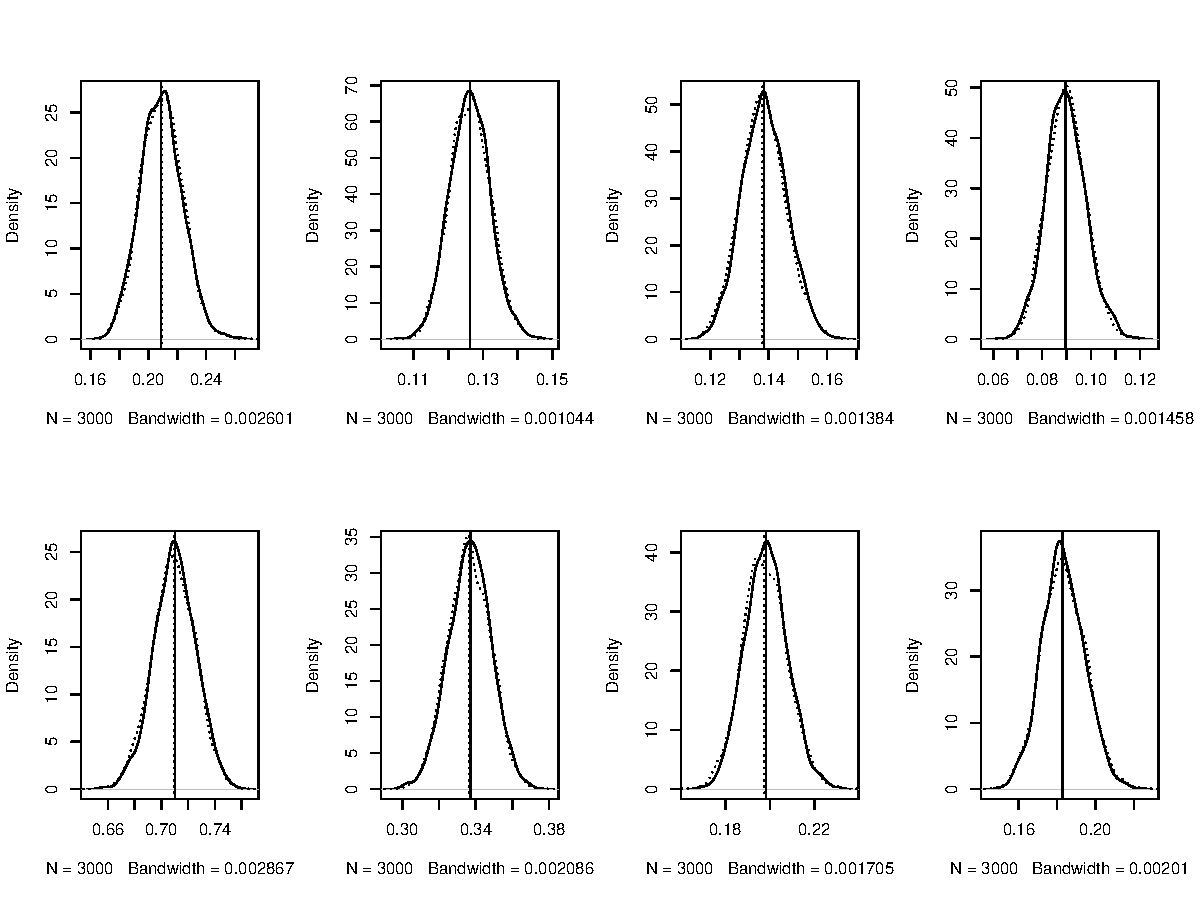
\includegraphics[page=1,width=.9\textwidth]{../figures/appendix-x-match}  
    \caption{ (A) This plot shows the posterior distribution of the beta-binomial parameterization with complete pooling (solid line) against the posterior distribution of the beta-binomial parameterization with partial pooling (dotted line). The medians are given by vertical lines. These are 8 population- and year- combinations that have 30 data points each. These correspond to points on the right side of Figure~\ref{fig:complete_vs_partial}. }
 \label{fig:match}
\end{figure}

 \begin{figure}[h]
   \centering
  %#\begin{tabular}{@{}c@{\hspace{.5cm}}c@{}}
       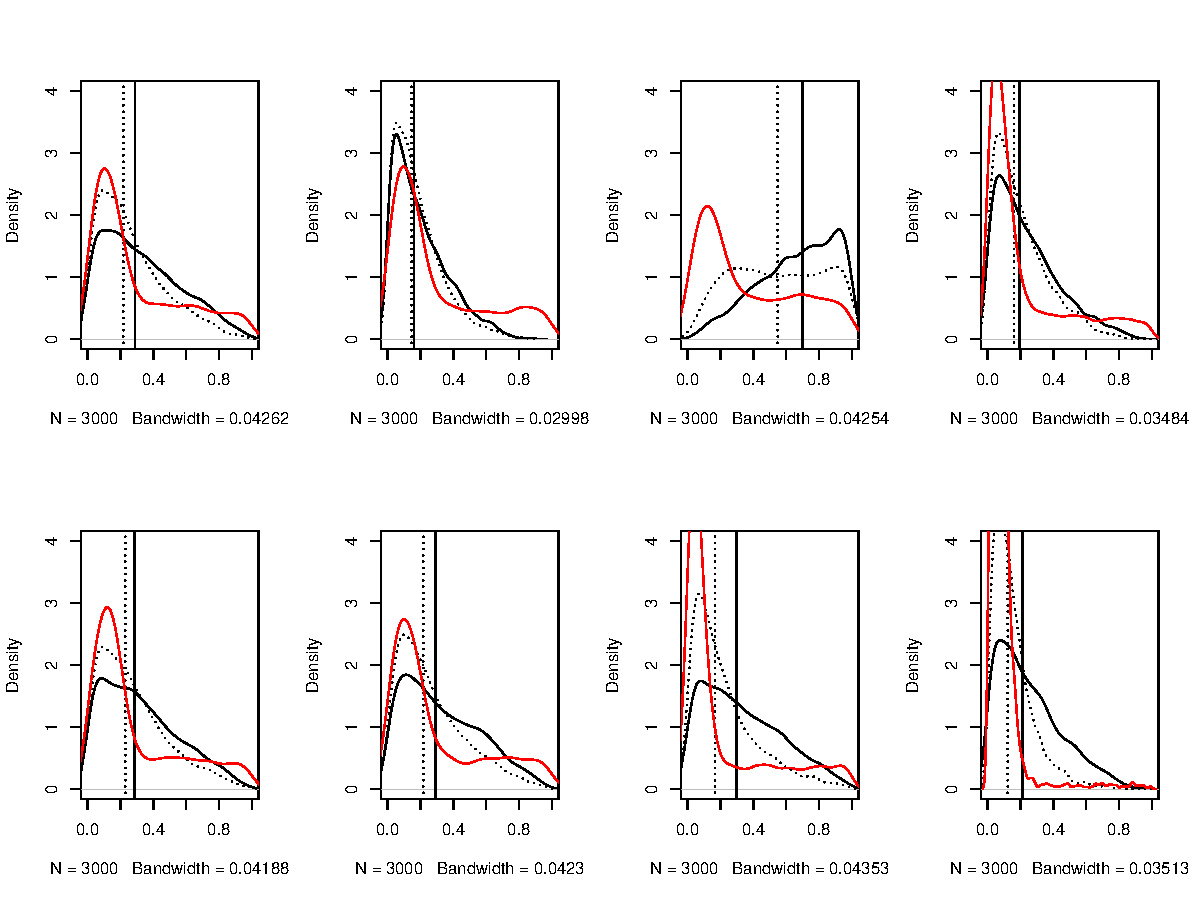
\includegraphics[page=1,width=.9\textwidth]{../figures/appendix-x-mismatch}  
    \caption{ (A) This plot shows the posterior distribution of the beta-binomial parameterization with complete pooling (solid line) against the posterior distribution of the beta-binomial parameterization with partial pooling (dotted line). The medians are given by vertical lines. The red lines are the population-level modes $\omega$. These are 8 population- and year- combinations that have only 1 data point each. These correspond to points on the left side of Figure~\ref{fig:complete_vs_partial}. }
 \label{fig:mismatch}
\end{figure}

 \begin{figure}[h]
   \centering
  %#\begin{tabular}{@{}c@{\hspace{.5cm}}c@{}}
       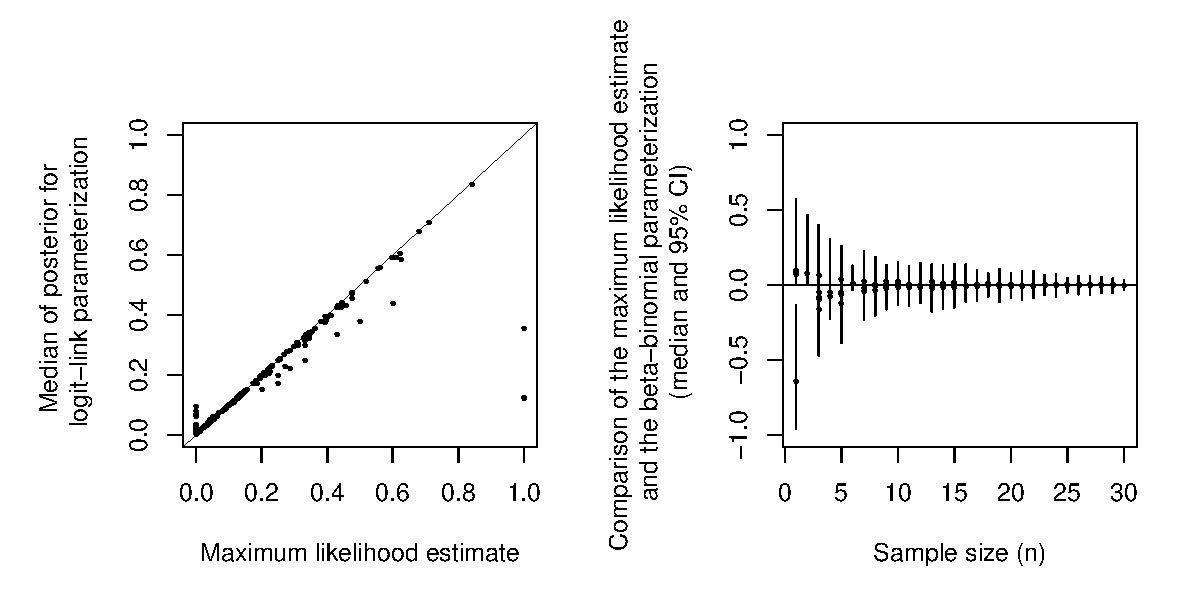
\includegraphics[page=1,width=.9\textwidth]{../figures/appendix-x-mle_bayeslogit}  
    \caption{ (A) This panel plots the median of the posterior from the logit parameterization with complete pooling per population against the maximum likelihood estimate. (B) This panel compares the full posterior distribution from the logit parameterization with the maximum likelihood estimate. The plot shows the median of the difference (with 95\% CIs) against the sample size in the year-population combination for that estimate. }
 \label{fig:logit}
\end{figure}

 \begin{figure}[h]
   \centering
  %#\begin{tabular}{@{}c@{\hspace{.5cm}}c@{}}
       \includegraphics[page=1,width=.9\textwidth]{../figures/appendix-x-bayescomp_bayeslogit}  
    \caption{ (A) This plot compares the full posterior distribution of the beta-binomial parameterization with complete pooling against the logit parameterization with compmlete pooling. The plot shows the median of the difference (with 95\% CIs) against the sample size in the year-population combination for that estimate.   }
 \label{fig:complete_vs_logit}
\end{figure}
\fi

  % BEGIN FIGURE 1
 \begin{tikzpicture}[
            > = stealth, % arrow head style
            shorten > = 1pt, % don't touch arrow head to node
            auto,
            node distance = 3cm, % distance between nodes
            semithick % line style
        ]

        \tikzstyle{every state}=[
            draw = none,
            thick,
            fill = white,
            minimum size = 4mm
        ]F


	% data level
        \node[state] (Y) [] {$y_i$};
        \node[state] (N) [right of=Y] {$n_i$};
       
        \path[dashed,->] (N) edge node {} (Y);

	% probability
        \node[state] (T) [below of = Y] {$\theta_i$};
                
         \path[->] (T) edge node {} (Y);
         
         % hyperparameters
         \node[state] (MN) [below of = T] {$\mu,\nu$};
                
         \path[->] (MN) edge node {} (T);
         
  \end{tikzpicture} 
  \hspace{1cm}% NO SPACE!
  % BEGIN FIGURE 2
   \begin{tikzpicture}[
            > = stealth, % arrow head style
            shorten > = 1pt, % don't touch arrow head to node
            auto,
            node distance = 3cm, % distance between nodes
            semithick % line style
        ]

        \tikzstyle{every state}=[
            draw = none,
            thick,
            fill = white,
            minimum size = 4mm
        ]F


	% data level
        \node[state] (Y) [] {$y_i$};
        \node[state] (N) [right of=Y] {$n_i$};
       
        \path[dashed,->] (N) edge node {} (Y);

	% probability
        \node[state] (T) [below of = Y] {$\theta_i$};
                
         \path[->] (T) edge node {} (Y);
         
         % hyperparameters
         \node[state] (AB) [below of = T] {$\phi, \kappa$};
                
         \path[->] (AB) edge node {} (T);
         
  \end{tikzpicture}
  
  % BEGIN FIGURE 3
   \begin{tikzpicture}[
            > = stealth, % arrow head style
            shorten > = 1pt, % don't touch arrow head to node
            auto,
            node distance = 3cm, % distance between nodes
            semithick % line style
        ]

        \tikzstyle{every state}=[
            draw = none,
            thick,
            fill = white,
            minimum size = 4mm
        ]F


	% data level
        \node[state] (Y) [] {$y_i$};
        \node[state] (N) [right of=Y] {$n_i$};
       
        \path[dashed,->] (N) edge node {} (Y);

	% probability
        \node[state] (T) [below of = Y] {$\theta_i$};
                
         \path[->] (T) edge node {} (Y);
         
         % hyperparameters
         \node[state] (AB) [below of = T] {$\alpha_i$};
                
         \path[->] (AB) edge node {} (T);
         
         % hyperparameters
         \node[state] (MS) [below of = AB] {$\mu, \sigma$};
                
         \path[->] (MS) edge node {} (AB);
         
  \end{tikzpicture}
  \hspace{1cm}% NO SPACE!
  % BEGIN FIGURE 3
   \begin{tikzpicture}[
            > = stealth, % arrow head style
            shorten > = 1pt, % don't touch arrow head to node
            auto,
            node distance = 3cm, % distance between nodes
            semithick % line style
        ]

        \tikzstyle{every state}=[
            draw = none,
            thick,
            fill = white,
            minimum size = 4mm
        ]F


	% data level
        \node[state] (Y) [] {$y_i$};
        \node[state] (N) [right of=Y] {$n_i$};
       
        \path[dashed,->] (N) edge node {} (Y);

	% probability
        \node[state] (T) [below of = Y] {$\theta_i$};
                
         \path[->] (T) edge node {} (Y);
                  
                  % hyperparameters
         \node[state] (AB) [below of = T] {$\alpha_i$};
                
         \path[->] (AB) edge node {} (T);
         
          % hyperparameters
        
         \node[state] (MS) [below of = AB] {$\mu, \sigma$};
         \node[state] (A) [below right of = AB] {$\alpha_{std}$};
         
         \path[->] (A) edge node {} (AB);       
         \path[->] (MS) edge node {} (AB);       
                 
  \end{tikzpicture}

 \begin{figure}[h]
   \centering
  %#\begin{tabular}{@{}c@{\hspace{.5cm}}c@{}}
       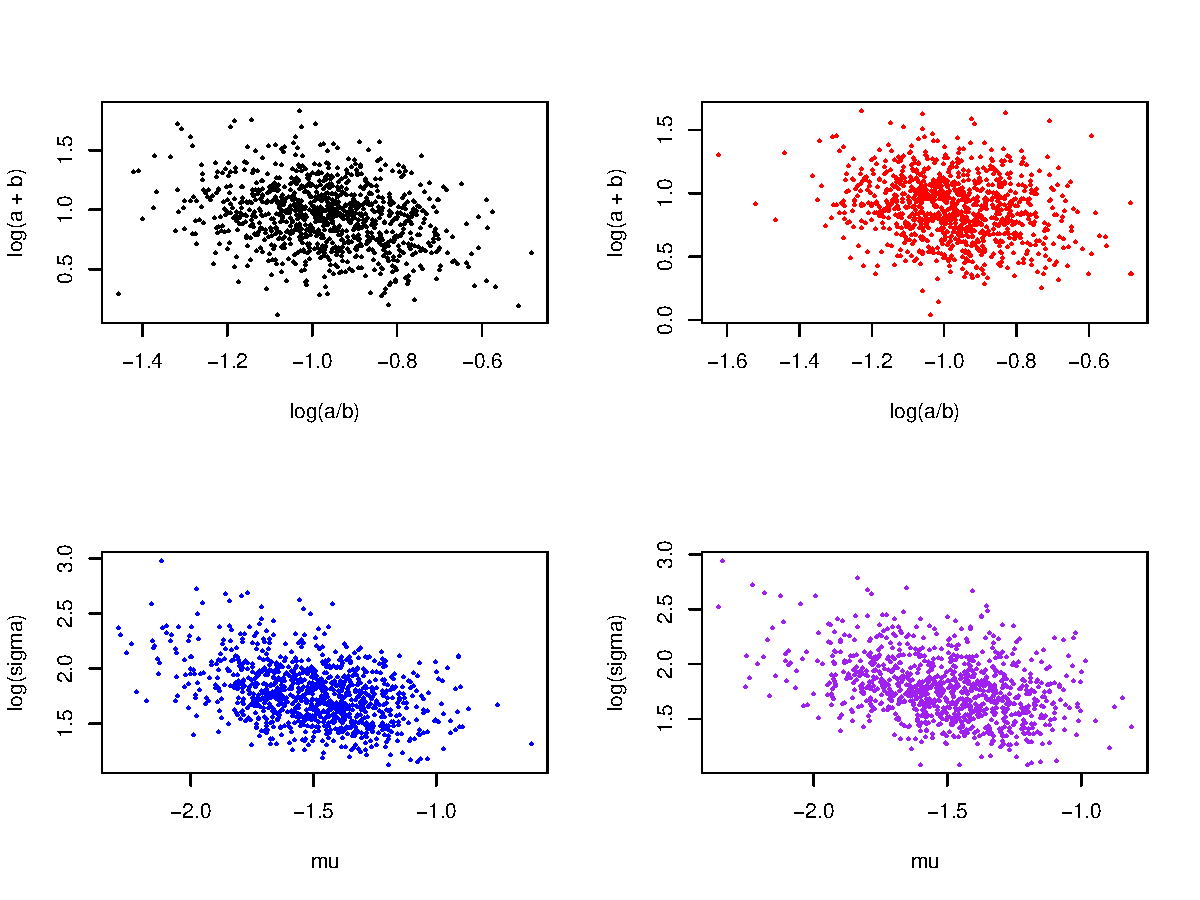
\includegraphics[page=1,width=.75\textwidth]{../figures/appendix/appendix-1/hyperparameterCorrelations}  
        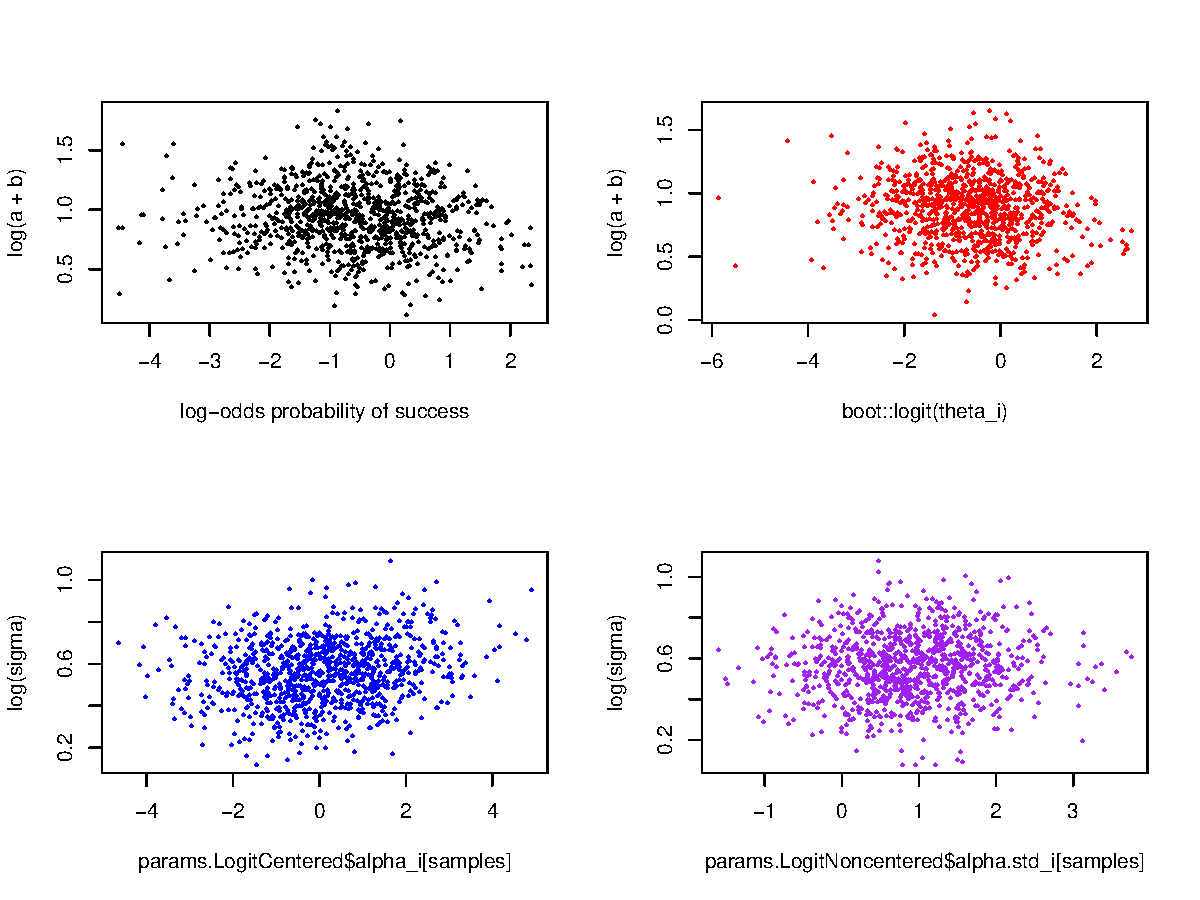
\includegraphics[page=1,width=.75\textwidth]{../figures/appendix/appendix-1/funnelCheck}  
    \caption{   }
 \label{fig:...}
\end{figure}


 \begin{figure}[h]
   \centering
  %#\begin{tabular}{@{}c@{\hspace{.5cm}}c@{}}
       \includegraphics[page=1,width=.9\textwidth]{../figures/appendix/appendix-1/neff}              
    \caption{   }
 \label{fig:...}
\end{figure}

 \begin{figure}[h]
   \centering
  %#\begin{tabular}{@{}c@{\hspace{.5cm}}c@{}}
       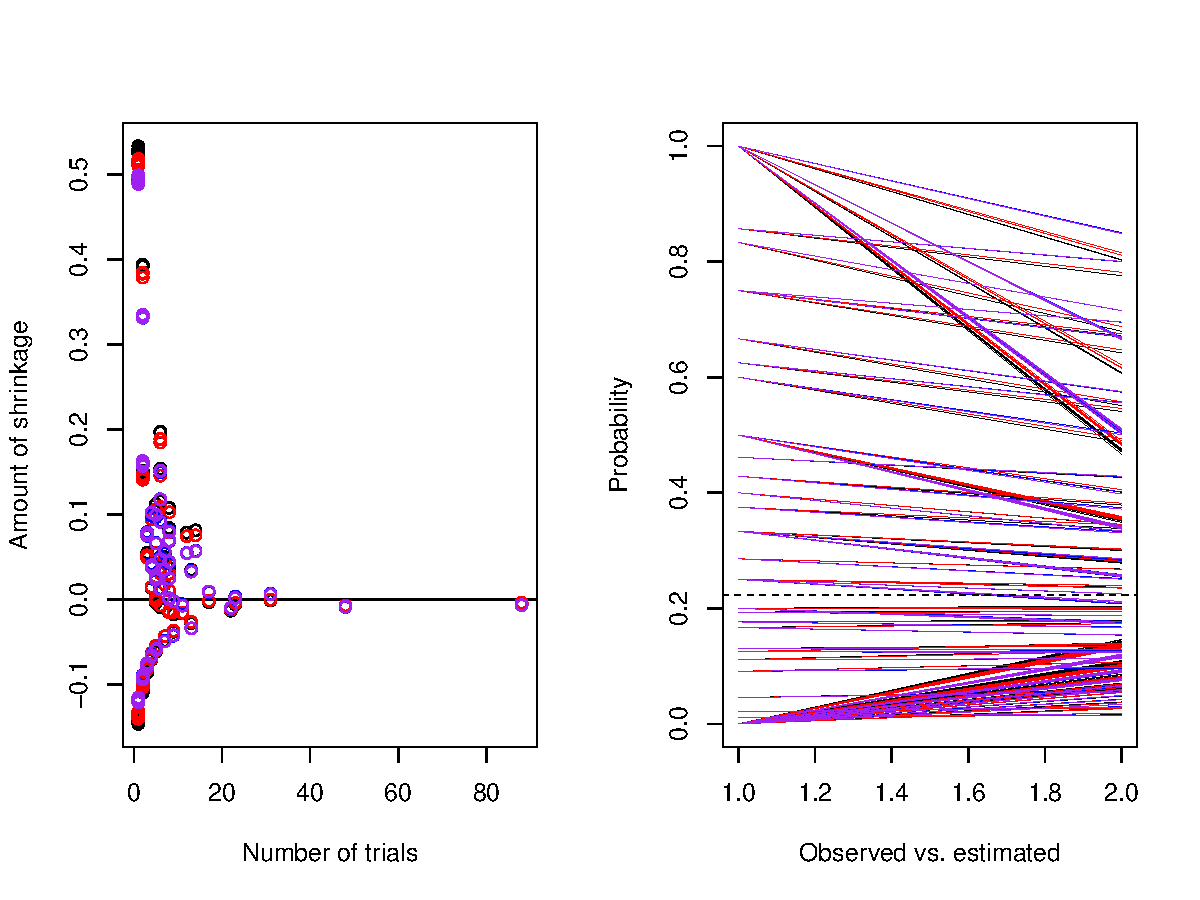
\includegraphics[page=1,width=.75\textwidth]{../figures/appendix/appendix-1/shrinkageSamplesize}              
    \caption{   }
 \label{fig:...}
\end{figure}

 \begin{figure}[h]
   \centering
  %#\begin{tabular}{@{}c@{\hspace{.5cm}}c@{}}
         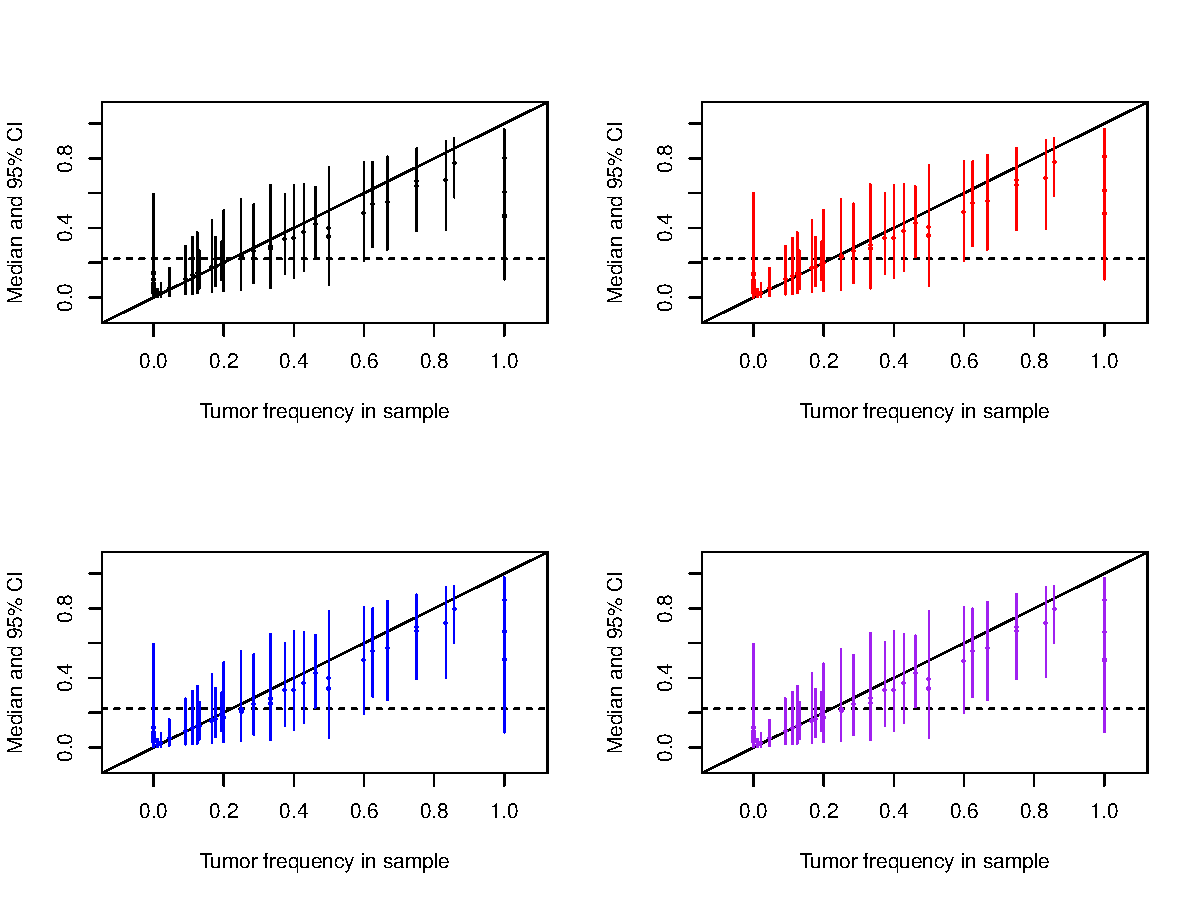
\includegraphics[page=1,width=.75\textwidth]{../figures/appendix/appendix-1/shrinkage}              
       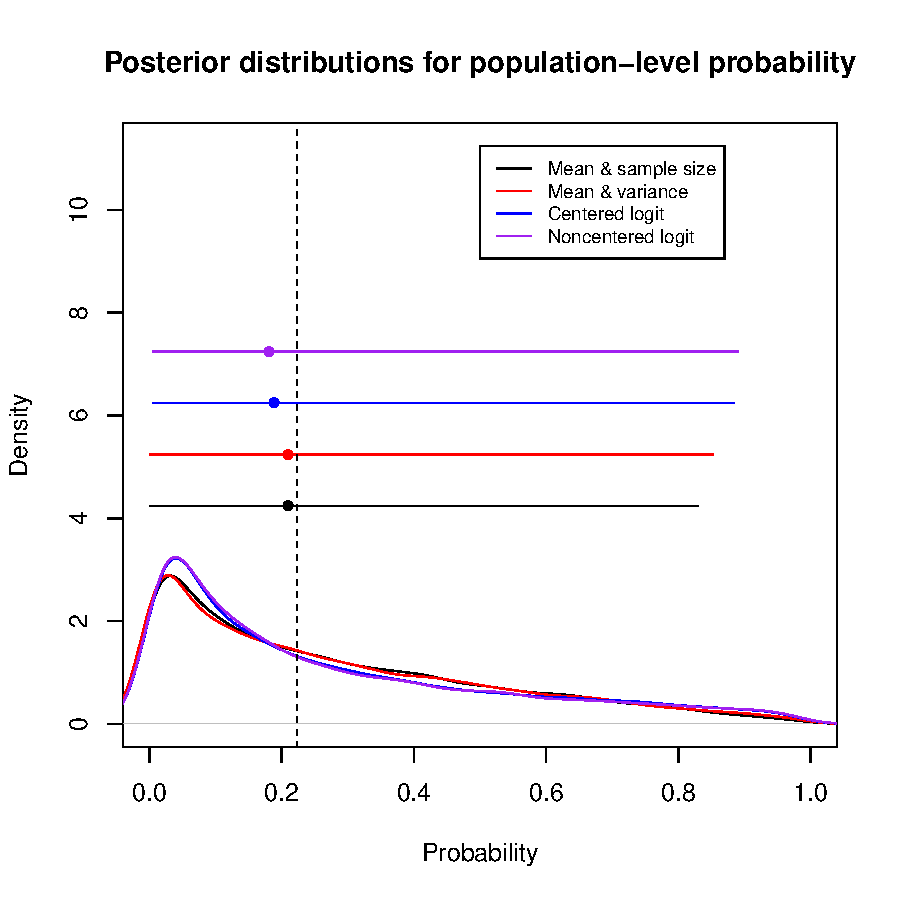
\includegraphics[page=1,width=.75\textwidth]{../figures/appendix/appendix-1/posteriorProbability}              
    \caption{   }
 \label{fig:...}
\end{figure}


\clearpage
\bibliography{/Users/gregor/Dropbox/bibliography/seeds}

\end{document}